
\documentclass[conference]{IEEEtran}
\IEEEoverridecommandlockouts
% The preceding line is only needed to identify funding in the first footnote. If that is unneeded, please comment it out.
\usepackage{cite}
\usepackage{amsmath,amssymb,amsfonts}
\usepackage{algorithmic}
\usepackage{graphicx}
\usepackage{textcomp}
\usepackage[ruled,vlined]{algorithm2e}
\usepackage{xcolor}
\def\BibTeX{{\rm B\kern-.05em{\sc i\kern-.025em b}\kern-.08em
    T\kern-.1667em\lower.7ex\hbox{E}\kern-.125emX}}
\begin{document}

\title{A Comprehensive Co-Evolutionary Framework for DNN Architecture Design Space Exploration on GPU Accelerator Platforms}

% \author{\IEEEauthorblockN{1\textsuperscript{st} Anand Ravishankar}
% \IEEEauthorblockA{\textit{Department of Electronics and Communications} \\
% \textit{BMSIT}\\
% Bangalore, India \\
% anandravishankar12@gmail.com}
% \and
% \IEEEauthorblockN{2\textsuperscript{nd} Santhi Natarajan}
% \IEEEauthorblockA{\textit{Department of Artificial Intelligence and Machine Learning} \\
% \textit{BMSIT}\\
% Bangalore, India \\
% santhi.natarajan@bmsit.in}
% \and
% \IEEEauthorblockN{3\textsuperscript{rd} Bharathi Malakreddy}
% \IEEEauthorblockA{\textit{Department of Artificial Intelligence and Machine Learning} \\
% \textit{BMSIT}\\
% Bangalore, India \\
% bharathi\_m@bmsit.in}
% }

\maketitle

\begin{abstract}

% Deep Neural Networks(DNNs) are an extremely attractive subset of computational models which provide promising results for a wide variety of problems. However, the performance delivered by DNNs overshadows the network architecture search(NAS) process and network's suitability for a given task. In this paper, we present an end-to-end framework designed to detect the abstract model required for a given data set, genetically modify the network architecture and evolve the knowledge representation format. The inherent parallelism offered by both the neural network and it's evolutionary extension is exploited by deploying the model on a GPU which substantially improves the throughput of Genetic-NAS.

Deep Neural Networks (DNNs) are an extremely attractive subset of computational models due to their remarkable ability to provide promising results for a wide variety of problems. However, the performance delivered by DNNs often overshadows the work done before training the network, which includes Network Architecture Search(NAS) and its suitability concerning the task. In this paper, we present a comprehensive end-to-end framework designed to detect the abstract model required for a given data set and genetically modify the network architecture and parameter set. Abstract model detection is done through a refinement subsystem which determines the modality of the data. The Genetic-NAS and parameter space exploration process is co-evolved by applying genetic operators and subjugating it to layer-wise competition. The inherent parallelism offered by both the neural network and its genetic extension is exploited by deploying the model on a GPU which substantially improves the throughput of Genetic-NAS.
  
\end{abstract}

\begin{IEEEkeywords}
Deep Nerual Networks, Network Architecture, Harware Acceleration, Co-evolutionary framework
\end{IEEEkeywords}

\section{Introduction}

Deep Neural Networks (DNNs) are parallel computational structures that implement static and dynamic systems through a process of knowledge accumulation rather than memorization. The steady rise in DNNs' popularity can be attributed to the influx of new architectures such as AlexNet\cite{AlexNet}, ResNet\cite{ResNet}, VGG\cite{VGG} and LSTM\cite{LSTM} among others, supplemented with a surge in hardware accelerators designed for parallel computation, such as GPUs, ASICs and FPGAs. Moreover, the algorithms governing the functionalities of the different neural networks have a strong underlying mathematical foundation, which has only reinforced over the years with Improved Back-Propogation \cite{IBP} and Conjugate Gradient Algorithm \cite{CGA} being prime examples. The performance (P) of a DNN can be expressed as a function of three main factors: network architecture (A), network parameter set (NP) and knowledge representation of the data provided (K).

\begin{equation}
P = \textit{f}(A, N\textsubscript{\textit{P}}, K) \label{performance}
\end{equation}

Much empahsis is placed on developing new algorithms and programming paradigms for modifying the network parameters to improve performance. With recent advances in GPU based accelerators, DNNs and Genetic Programming (GP) perform with an increased throughput, owing to their inherent parallelism. Multiple execution threads co-operate to complete the work in a shorter time frame. The MPI and CUDA frameworks allow interleaving of compute and data transfer I/O operations, resulting in an optimized performance. This overwhelming infatuation towards performance enhancement has often undermined the importance of network architecture selection and its association with the dataset provided. Given no prior knowledge, the Network Architecture Search (NAS) process has been a trivial trial-and-error process, which is painstakingly human. Moreover, given a network architecture and an optimized parameter set, the configuration stands good only for a given dataset and does not account for an runtime model with wild flucuations in the admitted dataset. Modern NAS techniques can be subdivided into Reinforcement Learning (RL) based, such as \cite{RLNAS1} and \cite{RLNAS2}, Evolutionary Techniques, such as \cite{ENAS}, and Gradient based Techniques, such as \cite{GNAS}. RL techniques suffer a high computational cost for combing through the entire search space and adapting to the environment, while Gradient based techniques are not adaptive in nature and hence cannot be applied to a runtime model. Applying a random search on network architecture would be time consuming and computationally expensive as the total number of configurations grow exponentially with even minor changes to the architecture. Thus, the existing solutions face the shortcomings listed below, that shall affect the system performance:

\begin{itemize}
\item Most systems are data set specific, and need to be re-engineered for a new application.
\item A new perturbation in the architecture space shall demand a fresh build of the whole system, rendering them outdated.
\item Pre-defined mathematical functions such as ReLu are static and do not keep up with the evolving search space.
\end{itemize}
In this paper, we present a dynamic end-to-end framework composed of intelligent subsystems, each one tackling one aspect of general DNNs' performance as stated in Equation $\ref{performance}$ to overcome the aforementioned shortcomings. The key features of our framework are:

\begin{itemize}
\item \textbf{Data Aware Model Selection}: A robust subsystem accepts the data either in the form of a single file or a directory and proposes a base model. The data is initially parsed through various signals such as polynomial features, temporal differences, spatial differences, dimensionality analysis and data formats. The queued data is assigned flags based on the signal results obtained. Further, an optimized scheduler limits the time difference between successive data admissions resulting in increased throughput.  
\item \textbf{Pattern Aware Pruning}: After selecting a base model for the task, genetic programming is introduced to grow out the model to its optimal structure. In order to limit the growth of the transition matrix, pruning is applied to the genetic structure so formed. The pruning areas are determined by applying Back Propogation (BP) and Markov chain analysis to the transition matrix and the corresponding pobabilistic states. 
\item \textbf{Layer-wise Competition}: For each layer, multiple instances are created and the fitness of each instance is evaluated after every iteration. The Genetic-NAS process is shifted away from an accuracy-driven model and special emphasis is given to the individual contributions of each instance.  
\end{itemize}

\section{Related Work}

Recent efforts of integrating multi-disciplinary algorithms with NAS has given rise to a copius amount of techniques to automate the search process. As mentioned previously, the efforts can be broadly classified as RL based, Evolutionary algorithm based and Gradient based techniques. RL based techniques treat the entire search space as a learning environment with parameter matrix of each layer's instance having either a positive or negative feedback. An external agent is employed to roam the search space and experience the environment, based on a pre-decided reward system. Evolutionary algorithms can be further sub-classified into Evolutionary Programming (EP) and Genetic Programming (GP). Both paradigms attempt to emulate Darwin's theory of evolution from different approaches with the help of genetic operators such as selection, crossover and mutation. Gradient based techniques utilize the gradient descent algorithm to test the goodness-of-fit of each layer's parameter.  

\begin{itemize}
\item \textbf{RL based}: In \cite{RWRL1} the authors generate high-performing CNN architectures for a given learning task using Q-learning with an $\epsilon$-greedy exploration strategy and experience replay; In \cite{RWRL2} the authors formulate the NAS as a Markov decision process which enables a more effective RL-based search. The samples generated by the previous policies are used efficiently for an off-policy GAN search algorithm.
\item \textbf{Evolutionary based}: In \cite{EA1} the authors construct a simplified supernet where all architectures are single paths which solves the weight co-adaption problem. Conduction of the search process in complex environments under multiple constraints is cnoducted seamlessly through uniform path sampling. In \cite{EA2} evolved machine learning algorithms are created from scratch. They apply evolutionary concepts on top of top algorithms such as bilinear interactions, normalized gradients, and weight averaging. In \cite{lund} a Genetic Algorithm (GA) is used to evolve ecological neural networks that can adapt to their changing environment. In \cite{hass} and \cite{munro}, a GA is used on a fixed three layer feedforward network to find the optimal mapping from the input to the hidden layer (i.e. the set of optimal hidden targets). 
\item \textbf{Gradient based}: Using Gradient descent offers a big advantage in terms of reduced GPU-hours as shown by \cite{GD1}. The entire search space is represented in the form of directed acyclic graphs each one of which constitutes a possible network architecture. A differential sampler is then trained through gradient descent which optimizes the learning process. The resultant network took only 4 GPU hours with a test error of 2.82\%. Another method involved optimizing the network configuration through stochastic relaxation as shown by \cite{GD2}. The authors apply gradient descent technique with adaptive step-size method for low cost computations.    



\end{itemize}

\begin{algorithm}[!t]
\scriptsize
\SetAlgoLined
Input: Training Set $D$, Fitness threshold $\lambda$, Base model $M$, Maximum Network Depth $max\_depth$, Maximum Nodes $max\_nodes$, Maximum Complexity $C$, Genetic Operators $G$\\
\KwResult{Optimal Network Configuration is obtained}\
------------------------------------------------------------
Initialize $I$ instances of Base Model with single block\;
Start initial run\;
\For{Each n in $max\_nodes$}{
    Develop the network under constraint $C$ and $max\_depth$;
    \For{Each instance $i$ in $I$}{
        Store fitness scores in array $scores$[];
    }
}
\For{Each Instance $i$ in $I$}{
Obtain Network configuration in an intermediate space through binary encoding;
Obtain $I$ chromosomes;
\For{Each potential solution chromosome in $I$}{
Establish a many-to-one relation with $w$ parameter representations\;
Using $G$ evolve the chromosome\;
}
Update $scores$[]\;
}
Translate the intermediate state to a binary evaulation tree\;
\For{Each node $n$ in chromosome $i$}{
Toggle the connection to the next layer using mutation\;
\If{Fitness score decreases}{
Apply Back propogation\;
Prune( Connection($i_n$) $->$ ($(i+1)_n$) );
}
\Else
{
\If{Any chromosome $i$ decreases below $\lambda$}
{break\;}
\Else
{continue\;}
}
}
\caption{Co-evolutionary NAS with parameter updation}
\label{alg1}
\end{algorithm}


\section{Co-Evolutionary NAS with network configuration optimization}

In this section, we dicuss the model selection process along with the co-evolutionary NAS and the corresponding GPU partitioning of the training phase. The goal of developing an end-to-end framework consists of three main components, each one focusing on one aspect of optimizing the performance of the base model. An additional component in the form of GPU implementation is added to provide a comparative study and to speed up the co-evolutionary NAS proccess. Note that a GPU-partitioned architecture has fewer weights because not all layers have interconnections. Dropping some of the interconnections through pruning reduces the communication time between the processors and therefore increases efficiency.
The end-to-end framework is described in Algorithm $\ref{alg1}$ and discussed in depth in the following subsections.



\subsection{\textbf{Base Model Selection}}
The overview of the model selection process is shown in Figure $\ref{part1}$.
\begin{figure}[!b]
\centerline{\includegraphics[width=50mm]{part1.png}}
\caption{Base Model Selection}
\label{part1}
\end{figure}

A central data repository is created for data admission and for each data entry, flags are initialised as null vectors. Depending on the workload provided, each entry is scheduled as a job and sequenced for processing. A non-preemptive approach is applied to the scheduling task for higher throughput and low scheduling overhead. The scheduler automates the tedious part of Machine Learning by intelligently exploring multiple pipelines to find the most apt one for the dataset provided. Once the jobs are optimally sequenced, they pass through a set of filters. These filters provide information about the job in terms of:

\begin{itemize}
\item Polynomial features
\item Dimensionality
\item Temporal dependencies
\item Spacial dependencies
\item Stacking Estimation
\end{itemize}

The filtered output has multiple feedback passes into the repository, where the flags are updated. Based on the flag configuration, a base model is proposed and is fed into the next subsystem along with the data. 

\subsection{\textbf{Genetic Programming based NAS and weight optimization}}

Once a base model such as Convolutional Neural Network (CNN) or Feed-Forward Network (FNN) is selected, GP is applied to build upon the base model. The general flow of this growth for a CNN is shown in Figure $\ref{part2}$. 

\begin{figure}[!b]
\centerline{\includegraphics[width=85mm]{part2.png}}
\caption{Genetic Programming based NAS}
\label{part2}
\end{figure}

A complementary co-dependent structure for optimizing the NAS process and the weight selection is employed using structured chromosomes in the representational space. For computational purposes, an intermediate state of binary matrix encoding is introduced. An n-dimensional matrix scheme has been implemented to represent the DNN structures in a concise manner. It encodes regularities in the connectivity matrix defining the network structure. Another added advantage of the binary representation is the translation of genetic operators as structural changes in the network, which in turn depend on the chromosome layer they are acting on. A many-to-one mapping is employed between the architectural representation and the weight representation, to have a two-step verification of the goodness-of-fit of the model as shown in Figure $\ref{part3}$.

\begin{figure}[!b]
\centerline{\includegraphics[width=85mm]{part3.png}}
\caption{Many-to-one relation between NAS and weight representation}
\label{part3}
\end{figure}
\subsubsection{\textbf{Pruning}}
In the evaluation stage of the encoding system, the generated networks are first pruned before they are trained, using the BP module. Pruning removes neurons and the corresponding links that have no incoming or outgoing connections. It does this recursively until all such neurons have been removed. BP training is performed for a predefined number of cycles, rather than the more customary process of stopping at a required error level, since network convergence is dependent on the network's configuration. The optimal number depends on the dataset provided and the train-test split set used. The BP module is a standard one using the normal gradient descent weight updating rule with a momentum term. The module uses a per-pattern weight update mechanism, meaning that the weights are updated after every iteration of the training phase.

The fitness function used to evaluate the goodness-of-fit of the network instance is given by Equation $\ref{F}$ 
\begin{equation}
F = \frac{\hat{Y}-Y}{\sum_{i=0}^{N}O\textsubscript{i}} + \alpha\frac{C}{C\textsubscript{max}} + \mu P
\label{F}
\end{equation}
where $\hat{Y}$ is the target variable, $Y$ is the predicted output, $O\textsubscript{i}$ is the number of output classes, $C$ is the network complexity, $C\textsubscript{max}$ is the maximum complexity, $P$ is the fraction of the network pruned, $\alpha$ is the learning rate and $\beta$ is momentum.  Note that since the fitness function is directly proportional to the loss, the problem of optimizing the neural network is a minimization problem rather than the usual maximization problem. 

\subsubsection{\textbf{Markov Chain analysis}}

The most common methods for analysing genetic structures include Schema theorem, Price's theorem and building block hypothesis. The methods mentioned provide a good approximation of the genetic model and have been used often. Markov Chain analysis however, replicates an exact model of the genetic structure in a state space diagram. The models so formed provide useful insight about the effect of genetic operators on the transition matrix.  

Since binary encoding was employed, the chromosomes are treated as binary strings with each gene representing "no connection" or 0 and "connection" or 1. If $N$ chromosomes of lenth $l$ are generated, the number of possible states are $N+1$. State $i$ is referred to as the state with exactly $i$ ones and $(l - i)$ zeros. The operation of the genetic algorithm is now defined by a $(l + 1)*(l + 1)$ transition matrix $P[i, j]$ that maps the current state $i$ to the next state $j$ . The probability of a transition from state $i$ to state $j$ is given by one
entry in the matrix $p(ij)$. A sample markov model for $l$ = 1 and $N$ = 4 is shown in Figure $\ref{part4}$.

\begin{figure}[!b]
\centerline{\includegraphics[width=50mm]{part4.png}}
\caption{Markov Analysis}
\label{part4}
\end{figure}

If $f\textsubscript{0}$ is the fitness of the chromosome of length $l$ having $i$ zeros, when the connection is severed and $f\textsubscript{1}$ is the fitness of the chromosome when the connection is retained, the probability of the connection surviving is given by Equation $\ref{prob1}$.

\begin{equation}
p\textsubscript{1} = \frac{i*f\textsubscript{1}}{i*f\textsubscript{1} + (l-i)*f\textsubscript{0}}
\label{prob1}
\end{equation}

And the probability of connection not surviving is given by Equation $\ref{prob2}$.

\begin{equation}
p\textsubscript{0} = \frac{(l-i)*f\textsubscript{0}}{i*f\textsubscript{1} + (l-i)*f\textsubscript{0}}
\label{prob2}
\end{equation}

Hence the probability of transition from state $i$ to $j$ can be written as:

\begin{equation}
p(i,j) = {l \choose j}(p\textsubscript{1})\textsuperscript{j}(p\textsubscript{0})\textsuperscript{l-j}\\
\label{prob3}
\end{equation}

Equation $\ref{prob3}$ completely discribes the transition matrix with no preference for a state( i.e. a population) with all-ones or a state with all-zeros, and the equation reduces to the one for pure genetic drift.

\section{Experimental Results}

In this section, we describe the experimental setup and follow it up with a discussion of results. We have implemented the GP algorithm for the NAS process. We have used evolutionary operators, along with BP, for parameter setting and network convergence. The rig setup for our experiment consisted of an Intel(R) Core(TM) Xeon Silver 4208 CPU@2.50GHz with 32GB RAM. We developed the DNN through Tensorflow v2.3 and deployed it on a HPC system with PowerEdge R740 motherboard and 1 NVIDIA Tesla V100-PCIe GPU card (5120 CUDA cores with a peak throughput of 112 TFLOPS). We conducted the experiments on six public datasets: MNIST digit classification \cite{mnist}, CIFAR-10, CIFAR-100 \cite{cifar}, Boston Housing price regression dataset \cite{boston}, IMDB movie review sentiment dataset \cite{IMDB} and Reuters newswire classification dataset \cite{reuters}. The network settings are described in Table $\ref{tab1}$.

\begin{table}[htbp]
\caption{Network Settings}
\begin{center}
\begin{tabular}{ c  c }
\hline
\textbf{Parameter}&\textbf{Setting}\\
\hline
\hline
{Learning Rate}&{X $\in$ [0.0001-1.0]}\\
\hline
{Momentum}&{X $\in$ [0.0-0.9]}\\
\hline
{Back Propogation Cycles}&{$<$50}\\
\hline
{Encoding}&{Binary}\\
\hline
{Selection}&{Elitism}\\
\hline
{Mutation}&{Binary Inversion}\\
\hline
{Crossover}&{Single Point}\\
\hline
{Mutation Rate}&{X $\in$ [0.0-1.0]}\\
\hline
{Crossover Rate}&{X $\in$ [0.001-1.0]}\\
\hline
{Maximum Depth}&{5}\\
\hline
{Maximum Nodes}&{1024}\\
\hline
{$l$}&{31}\\
\hline
{$N$}&{10}\\
\hline
{Number of Generations}&{10}\\
\hline
{Number of epochs}&{10}\\
\hline
{Replacement}&{Unconditional}\\
\hline
% \textbf{Table}&\multicolumn{3}{|c|}{\textbf{Table Column Head}} \\
% \cline{2-4} 
% \textbf{Head} & \textbf{\textit{Table column subhead}}& \textbf{\textit{Subhead}}& \textbf{\textit{Subhead}} \\
% \hline
% copy& More table copy$^{\mathrm{a}}$& &  \\
% \hline
% \multicolumn{4}{l}{$^{\mathrm{a}}$Sample of a Table footnote.}
\end{tabular}
\label{tab1}
\end{center}
\end{table}


\subsubsection{Model selection}

We conducted the initial experiments on text based datasets i.e, \cite{IMDB}, \cite{reuters} and \cite{boston}. The datasets were admitted one by one and the respective flags were initialized to null vectors. The filter set described in the previous section is utilized to search through the possible avenues for our data to traverse through. The dataset is passed through the filter set for 10 cycles which cements the tuning result. Note that the dataset is passed through the filters in a divided format in order to prevent over-saturation of the filter output. The number of divisions in the sampled dataset is equal to the number of cycles. The throughput percentage for text based datasets (Orange) and image based datasets (Blue) is shown in Figure $\ref{throughput_pct}$. 

\begin{figure}[!b]
\centerline{\includegraphics[width=85mm]{throughput_pct.png}}
\caption{Throughput \% vs Number of Cycles}
\label{throughput_pct}
\end{figure}

\subsubsection{Genetic-NAS}

Both the structural part of the chromosomes and the connections use binary encoding. The coding of the structural part is, in general, non-homogeneous in that it consists of different parts, each having its own gene length. These parts correspond to the rewriting rules for one or more rewriting cycles. In the present implementation, only homogeneous chromosomes were used because implementing non-homogeneous chromosomes in core genetic programming is quite difficult. 

Figures $\ref{boston}$ and $\ref{10}$ show the relation between network configuration of the image dataset and text dataset systems and their binary encoded formats. Both systems showed very similar behaviour on this problem. Convergence curves of the best individual in the population versus generation were nearly identical as shown in the Image based Plots $\ref{conv_loss}$ (Red:MNIST, Blue:CIFAR-10, Green:CIFAR-100) and Text based Plots $\ref{text_loss}$ (Magenta: Boston, Green: IMDB, Red: Reuters). The resulting convergence proves the competence of the base model proposed. 
\begin{figure}[!b]
\centerline{\includegraphics[width=70mm]{boston.png}}
\caption{Boston dataset genomic encoding}
\label{boston}
\end{figure}

\begin{figure}[!b]
\centerline{\includegraphics[width=70mm]{cifar10.png}}
\caption{CIFAR10 dataset genomic encoding}
\label{10}
\end{figure}

\begin{figure}[!t]
\centerline{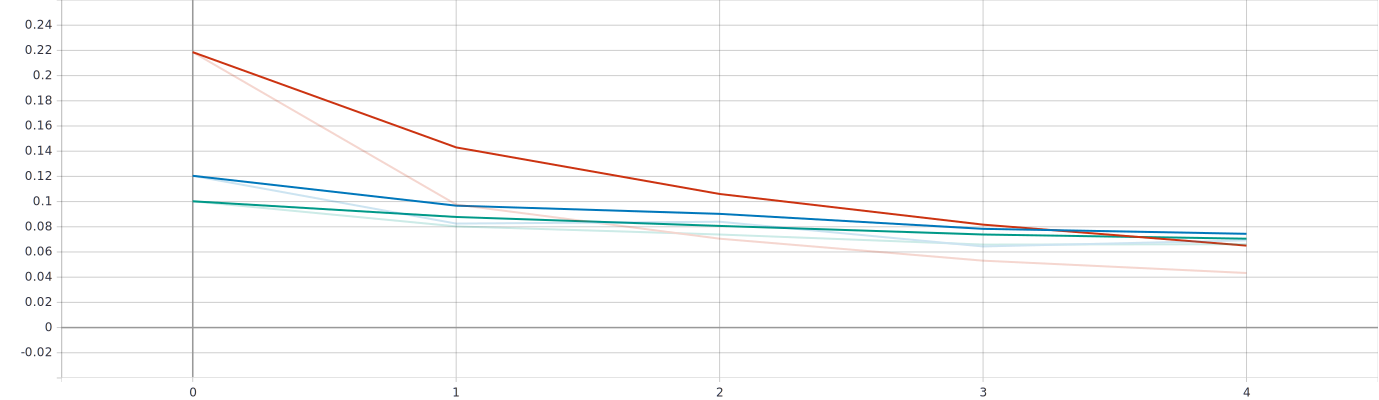
\includegraphics[width=90mm]{epoch_loss.png}}
\caption{Loss for Image based Datasets}
\label{conv_loss}
\end{figure}

\begin{figure}[!t]
\centerline{\includegraphics[width=90mm]{epoch_loss_2.png}}
\caption{Loss for Text based Datasets}
\label{text_loss}
\end{figure}

\subsubsection{Impact of Hardware Accelerators}

Due the parallel nature of DNNs, implementing them on GPUs reduces the average step time considerably. Moreover, genetic operations such as crossover and mutation can be applied in parallel as the operations are independent of the data involved. The placement of Tensorflow operations on a GPU device provides an acceleration of 8.4x with 92.9\% of the workload being placed on the GPU device. On an average, the task of classifying an image based dataset takes 3 GPU hours. The reduced time frame enables an increased throughput, while accelerating design space exploration process, as compared to a sequential search. 

\section{Conclusion and Future Work}

The proposed framework reads the dataset admitted and parses it along multiple filters. The filters in turn set flags indicating the nature of the datset admitted and proposes a base predictive model. The model is then co-evolved in terms of the network architecture and the parameters defining its configuration. The evolution is done with the help of genetic programming, which translates the actual configuration into a binary space representation. Genetic modifiers such as crossover, mutation and selection are now applied and the model is continously graded against a fitness funtion. Back propogation is applied to prune the network and reduce the growth of the binary encodings. 

The genetic components of our framework offer a wide array of advantages such as decrease in computational cost, avoidance of local optima and does not mandate an absolute representation of the network. However, due to the binary encoding system, the complexity increases exponentially as the size of the problem increases. This issue is, to a great extent, addressed by the introduction of a hardware accelerator. Additional improvements can be made to this project in terms of finer filters, amalgamation of co-evolution with RL for improved performance and introduction of new baseline architectures.  
% 
% \subsection{Units}
% \begin{itemize}
% \item Use either SI (MKS) or CGS as primary units. (SI units are encouraged.) English units may be used as secondary units (in parentheses). An exception would be the use of English units as identifiers in trade, such as ``3.5-inch disk drive''.
% \item Avoid combining SI and CGS units, such as current in amperes and magnetic field in oersteds. This often leads to confusion because equations do not balance dimensionally. If you must use mixed units, clearly state the units for each quantity that you use in an equation.
% \item Do not mix complete spellings and abbreviations of units: ``Wb/m\textsuperscript{2}'' or ``webers per square meter'', not ``webers/m\textsuperscript{2}''. Spell out units when they appear in text: ``. . . a few henries'', not ``. . . a few H''.
% \item Use a zero before decimal points: ``0.25'', not ``.25''. Use ``cm\textsuperscript{3}'', not ``cc''.)
% \end{itemize}
% 
% \subsection{Equations}
% Number equations consecutively. To make your 
% equations more compact, you may use the solidus (~/~), the exp function, or 
% appropriate exponents. Italicize Roman symbols for quantities and variables, 
% but not Greek symbols. Use a long dash rather than a hyphen for a minus 
% sign. Punctuate equations with commas or periods when they are part of a 
% sentence, as in:
% \begin{equation}
% a+b=\gamma\label{eq}
% \end{equation}
% 
% \subsection{Some Common Mistakes}\label{SCM}
% \begin{itemize}
% \item The word ``data'' is plural, not singular.
% \item The subscript for the permeability of vacuum $\mu_{0}$, and other common scientific constants, is zero with subscript formatting, not a lowercase letter ``o''.
% \item In American English, commas, semicolons, periods, question and exclamation marks are located within quotation marks only when a complete thought or name is cited, such as a title or full quotation. When quotation marks are used, instead of a bold or italic typeface, to highlight a word or phrase, punctuation should appear outside of the quotation marks. A parenthetical phrase or statement at the end of a sentence is punctuated outside of the closing parenthesis (like this). (A parenthetical sentence is punctuated within the parentheses.)
% \item A graph within a graph is an ``inset'', not an ``insert''. The word alternatively is preferred to the word ``alternately'' (unless you really mean something that alternates).
% \item Do not use the word ``essentially'' to mean ``approximately'' or ``effectively''.
% \item In your paper title, if the words ``that uses'' can accurately replace the word ``using'', capitalize the ``u''; if not, keep using lower-cased.
% \item Be aware of the different meanings of the homophones ``affect'' and ``effect'', ``complement'' and ``compliment'', ``discreet'' and ``discrete'', ``principal'' and ``principle''.
% \item Do not confuse ``imply'' and ``infer''.
% \item The prefix ``non'' is not a word; it should be joined to the word it modifies, usually without a hyphen.
% \item There is no period after the ``et'' in the Latin abbreviation ``et al.''.
% \item The abbreviation ``i.e.'' means ``that is'', and the abbreviation ``e.g.'' means ``for example''.
% \end{itemize}
% An excellent style manual for science writers is \cite{b7}.

% 
% \begin{table}[htbp]
% \caption{Table Type Styles}
% \begin{center}
% \begin{tabular}{|c|c|c|c|}
% \hline
% \textbf{Table}&\multicolumn{3}{|c|}{\textbf{Table Column Head}} \\
% \cline{2-4} 
% \textbf{Head} & \textbf{\textit{Table column subhead}}& \textbf{\textit{Subhead}}& \textbf{\textit{Subhead}} \\
% \hline
% copy& More table copy$^{\mathrm{a}}$& &  \\
% \hline
% \multicolumn{4}{l}{$^{\mathrm{a}}$Sample of a Table footnote.}
% \end{tabular}
% \label{tab1}
% \end{center}
% \end{table}
% 
% \begin{figure}[htbp]
% \centerline{\includegraphics{fig1.png}}
% \caption{Example of a figure caption.}
% \label{fig}
% \end{figure}

% 
\begin{thebibliography}{00}
\bibitem{AlexNet} Alex Krizhevsky, Ilya Sutskever, and Geoffrey E Hinton. 2012. ImageNet Classification with Deep Convolutional Neural Networks. In NIPS. 
\bibitem{ResNet}Kaiming He, Xiangyu Zhang, Shaoqing Ren, and Jian Sun. 2016. Deep residual learning for image recognition. In CVPR.
\bibitem{VGG} Karen Simonyan and Andrew Zisserman. 2015. Very Deep Convolutional Networks for Large-scale Image Recognition. In ICLR.
\bibitem{LSTM} Sepp Hochreiter; Jürgen Schmidhuber (1997). "Long short-term memory". Neural Computation. 
\bibitem{IBP} Nawi N.M., Ransing R.S., Salleh M.N.M., Ghazali R., Hamid N.A. (2010) An Improved Back Propagation Neural Network Algorithm on Classification Problems. In: Zhang Y., Cuzzocrea A., Ma J., Chung K., Arslan T., Song X. (eds) Database Theory and Application, Bio-Science and Bio-Technology. BSBT 2010, DTA 2010. Communications in Computer and Information Science, vol 118. Springer, Berlin, Heidelberg.
\bibitem{CGA} B. Wang, B. Yang, J. Sheng, M. Chen and G. He, "An Improved Neural Network Algorithm and its Application in Sinter Cost Prediction," 2009 Second International Workshop on Knowledge Discovery and Data Mining, Moscow, 2009, pp. 112-115, doi: 10.1109/WKDD.2009.180.
\bibitem{RLNAS1} Barret Zoph, Quoc V. Le, Neural Architecture Search with Reinforcement Learning, arXiv:1611.01578
\bibitem{RLNAS2} H. Liu and C. Zhang, "Reinforcement Learning based Neural Architecture Search for Audio Tagging," 2020 International Joint Conference on Neural Networks (IJCNN), Glasgow, United Kingdom, 2020, pp. 1-8, doi: 10.1109/IJCNN48605.2020.9207530.
\bibitem{ENAS} Clifford Broni-Bediako, Yuki Murata, Luiz Henrique Mormille, Masayasu Atsumi, Evolutionary NAS with Gene Expression Programming of Cellular Encoding, arXiv:2005.13110
\bibitem{GNAS} Liam Li, Mikhail Khodak, Maria-Florina Balcan, Ameet Talwalkar, Geometry-Aware Gradient Algorithms for Neural Architecture Search, arXiv:2004.07802
\bibitem{RWRL1} Baker B, Gupta O, Naik N, et al. Designing neural network architectures using reinforcement learning[J]. arXiv preprint arXiv:1611.02167, 2016
\bibitem{RWRL2} Yuan Tian, Qin Wang, Zhiwu Huang, Wen Li, Dengxin Dai1, Minghao Yang, Jun Wang, and Olga Fink, Off-Policy Reinforcement Learning for Efficientand Effective GAN Architecture Search. arXiv:2007.09180
\bibitem{EA1} Zichao Guo, Xiangyu Zhang, Haoyuan Mu, Wen Heng, Zechun Liu, Yichen Wei, Jian Sun, Single Path One-Shot Neural Architecture Search with Uniform Sampling, arXiv:1904.00420
\bibitem{EA2} Esteban Real, Chen Liang, David R. So, Quoc V. Le, AutoML-Zero: Evolving Machine Learning Algorithms From Scratch, arXiv:2003.03384

\bibitem{lund} Lund, H.H. and Parisi, D., "Simulations with an Evolvable Fitness Formula" Technical Report PCIA-1-94, C.N.R., Rome, 1994.
\bibitem{hass} Hassoun, M.H., Fundamentals of Artificial Neural Networks, MIT Press, 1995.
\bibitem{munro} Munro, P.W., "Genetic Search for Optimal Representations in Neural Networks", International Conference on Artificial Neural Nets and Genetic Algorithms (ANNGA93), Innsbruck, Austria, pp. 628-634, 1993.
\bibitem{GD1} Xuanyi Dong, Yi Yang Searching for A Robust Neural Architecture in Four GPU Hours. arXiv:1910.04465
\bibitem{GD2} Youhei Akimoto, Shinichi Shirakawa, Nozomu Yoshinari, Kento Uchida, Shota Saito, Kouhei Nishida, Adaptive Stochastic Natural Gradient Method for One-Shot Neural Architecture Search, arXiv:1905.08537
\bibitem{mnist} LeCun, Yann and Cortes, Corinna. "MNIST handwritten digit database." (2010): 
\bibitem{cifar} Learning Multiple Layers of Features from Tiny Images, Alex Krizhevsky, 2009.
\bibitem{boston} Harrison, D. and Rubinfeld, D.L. Hedonic prices and the demand for clean air, J. Environ. Economics and Management, vol.5, 81-102, 1978. 
\bibitem{IMDB} Andrew L. Maas, Raymond E. Daly, Peter T. Pham, Dan Huang, Andrew Y. Ng, and Christopher Potts. (2011). Learning Word Vectors for Sentiment Analysis. The 49th Annual Meeting of the Association for Computational Linguistics (ACL 2011).
\bibitem{reuters} Sam Dobbins, Mike Topliss, Steve Weinstein Reuters-21578, 1987
\end{thebibliography}
% \vspace{12pt}
% \color{red}
% IEEE conference templates contain guidance text for composing and formatting conference papers. Please ensure that all template text is removed from your conference paper prior to submission to the conference. Failure to remove the template text from your paper may result in your paper not being published.

\end{document}
